	%-----------------------
	\chapter{Réalisation}
	%-----------------------

Nous avons accompli notre objectif qui était de synchroniser les mouvements de plusieurs araignées 
entre elles grâce à Micro-ROS.
Une démo peut être consultée à cette adresse : \url{https://www.youtube.com/watch?v=Oyxngs2QC1o}.
\linebreak
L'araignée est contrôlée par une manette Xbox et il est possible d'augmenter ou diminuer la vitesse des mouvements en appuyant sur 
les joysticks.

		%-----------------------
		\section{Implémentation technique}
		%-----------------------

			%-----------------------
			\subsection{Les différences entre ROS et ROS2}
			%-----------------------

Une des principales différences entre ROS et ROS2 est leur architecture. ROS est basé sur une architecture monolithique, 
dans laquelle tous les composants logiciels sont intégrés dans un seul et même système d'exploitation. 
ROS2, en revanche, est basé sur une architecture modulaire, dans laquelle chaque composant logiciel peut être exécuté 
indépendamment des autres dans un système d'exploitation distribué. Cette architecture modulaire permet une meilleure flexibilité, 
une meilleure évolutivité et une meilleure tolérance aux pannes que l'architecture monolithique de ROS. 
\linebreak

Une autre différence importante entre ROS et ROS2 est leur modèle de communication. ROS utilise un modèle de communication basé 
sur le publisheur-abonné, dans lequel les composants logiciels peuvent envoyer et recevoir des données en utilisant des "topics" définis. 
ROS2, en revanche, utilise un modèle de communication basé sur les services et les requêtes, dans lequel les composants logiciels peuvent 
interagir en invoquant des services et en envoyant des requêtes. Ce modèle de communication permet une meilleure gestion des données et 
une meilleure flexibilité pour les applications de robotique. 
\linebreak

Enfin, ROS et ROS2 diffèrent également en termes de langages de programmation et de plateformes de développement. 
ROS prend en charge principalement le langage de programmation C++, bien qu'il soit également possible de l'utiliser avec d'autres 
langages tels que Python. ROS2 prend en charge plusieurs langages de programmation, tels que C++, Python, Java, et bien d'autres. 
De plus, ROS utilise principalement le système de build Catkin pour la compilation et l'intégration de logiciels, alors que 
ROS2 utilise l'outil de build Colcon. 

			%-----------------------
			\subsection{Les mouvements de l'araignée}
			\label{les_mouvements}
			%-----------------------

Nous avons implémenté les mouvements de l'arraignée pédagogique SEALK dont le code nous a été fourni. Voici la liste des différents mouvements :	

sit : fait asseoir l'arraignée

\begin{figure}[H]
	\begin{center}
		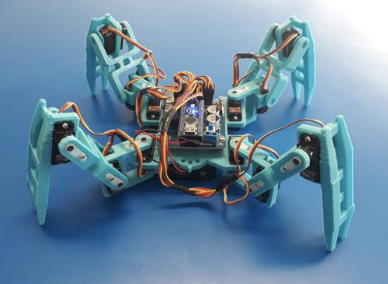
\includegraphics[width=0.3\textwidth]{./img/sit}
		\caption{Sit}
	\end{center}
\end{figure}

stand : met debout l'arraignée

\begin{figure}[H]
	\begin{center}
		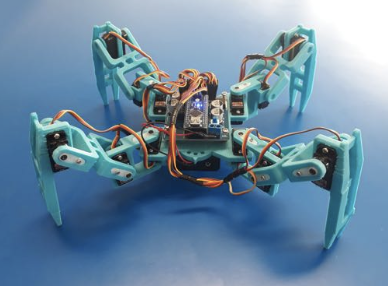
\includegraphics[width=0.3\textwidth]{./img/stand}
		\caption{Stand}
	\end{center}
\end{figure}

walk forward, walk back, walk left, walk right : bouge l'arraignée dans les quatre directions

\begin{center}
	\textit{pas d'image :(}
\end{center}

turn left, turn right : tourne l'araignée à gauche et à droite

\begin{figure}[H]
	\begin{center}
		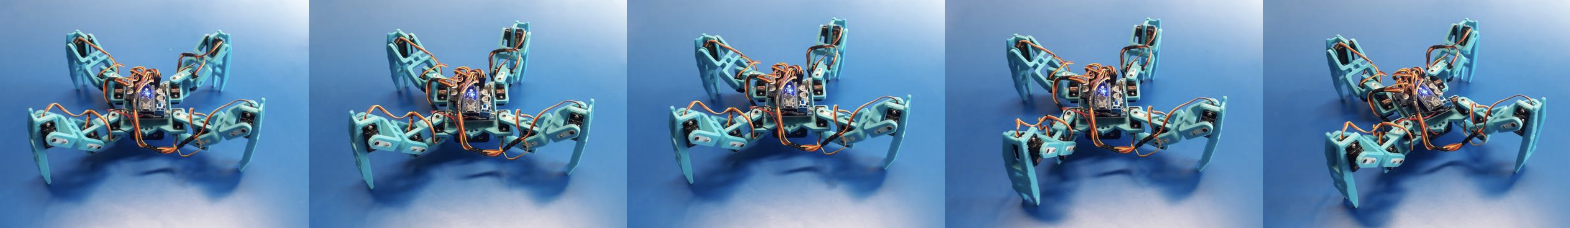
\includegraphics[width=0.8\textwidth]{./img/turn_left_1}
		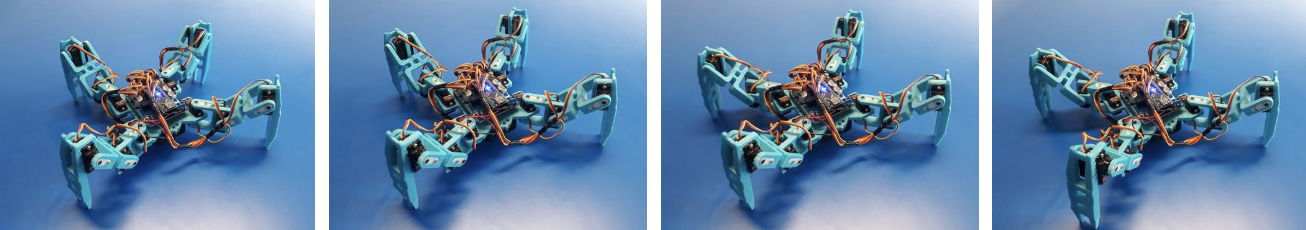
\includegraphics[width=0.8\textwidth]{./img/turn_left_2}
		\caption{Turn left}
	\end{center}
\end{figure}

rave : mouvement de divagation

\begin{figure}[H]
	\begin{center}
		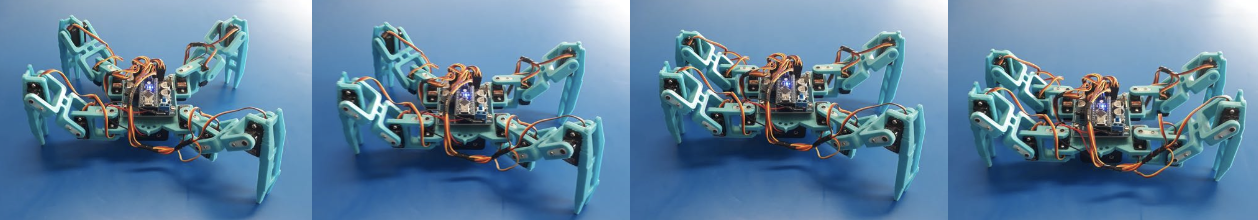
\includegraphics[width=0.8\textwidth]{./img/rave_1}
		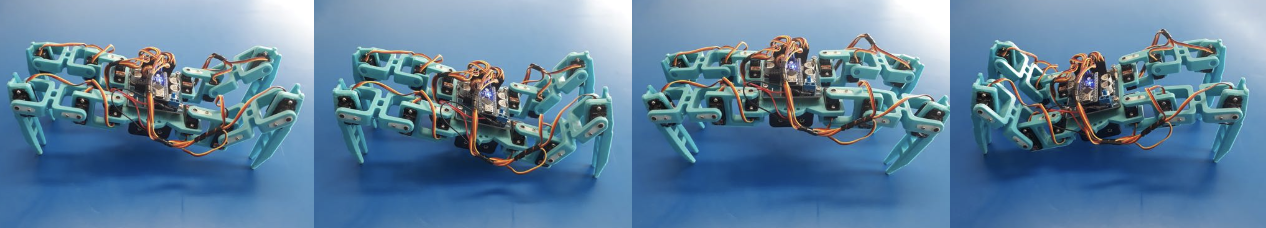
\includegraphics[width=0.8\textwidth]{./img/rave_2}
		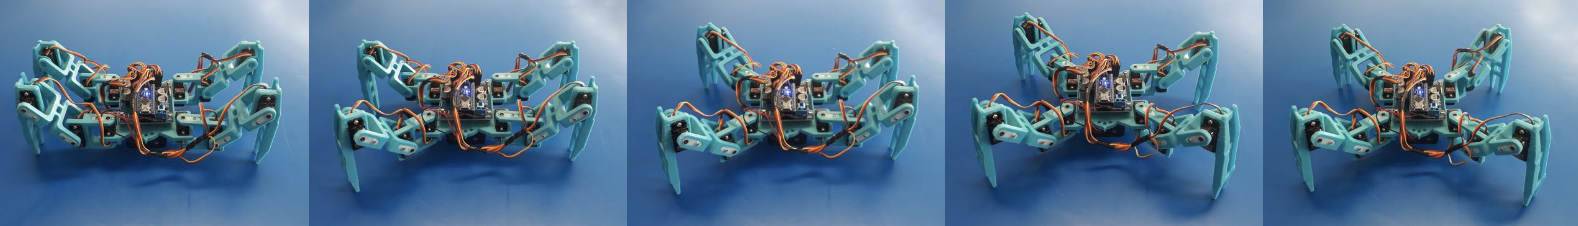
\includegraphics[width=0.8\textwidth]{./img/rave_3}
		\caption{Rave}
	\end{center}
\end{figure}

flex : fait un mouvement de "flex" au sol

\begin{figure}[H]
	\begin{center}
		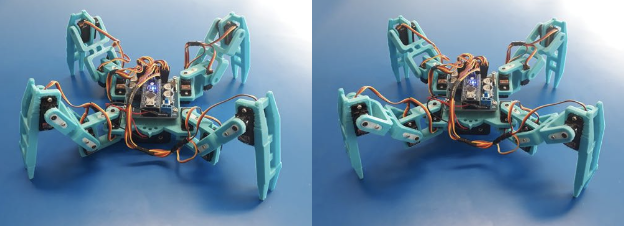
\includegraphics[width=0.6\textwidth]{./img/flex}
		\caption{Flex}
	\end{center}
\end{figure}

hello : fait un salut

\begin{figure}[H]
	\begin{center}
		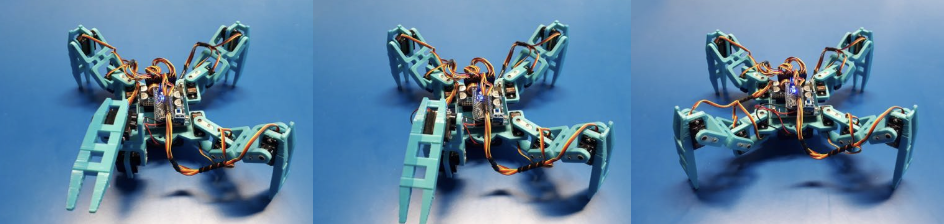
\includegraphics[width=0.6\textwidth]{./img/hello}
		\caption{Hello}
	\end{center}
\end{figure}

applaud sym : l'araignée simule un applaudissement en levant d'abord deux pattes en diagonale et les repose puis lève et 
repose les deux autres

\begin{figure}[H]
	\begin{center}
		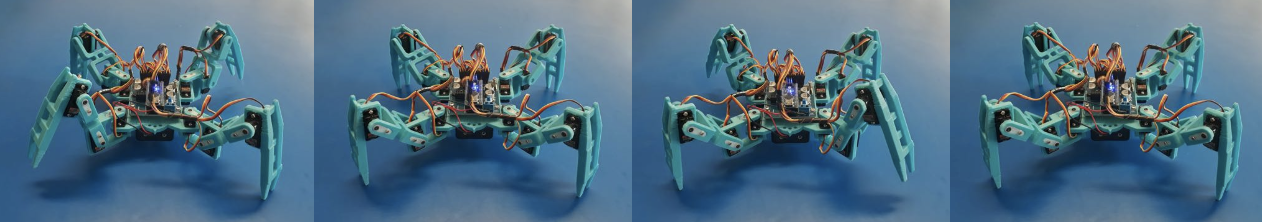
\includegraphics[width=0.6\textwidth]{./img/applaud_sym}
		\caption{Applaud sym}
	\end{center}
\end{figure}

applaud wave : similaire au mouvement précédent mais lève une seule patte à la fois

\begin{figure}[H]
	\begin{center}
		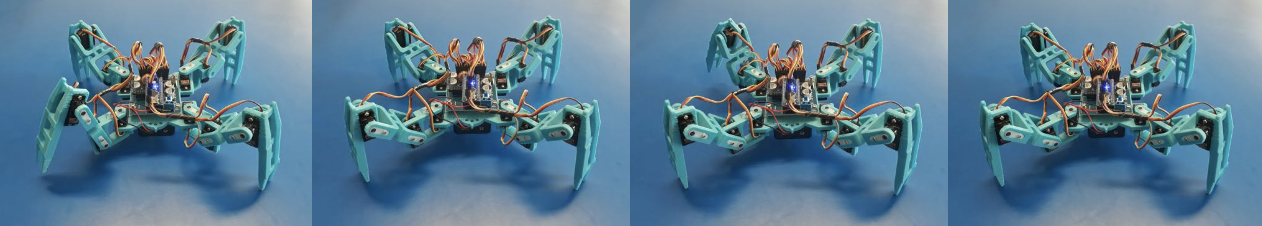
\includegraphics[width=0.8\textwidth]{./img/applaud_wave_1}
		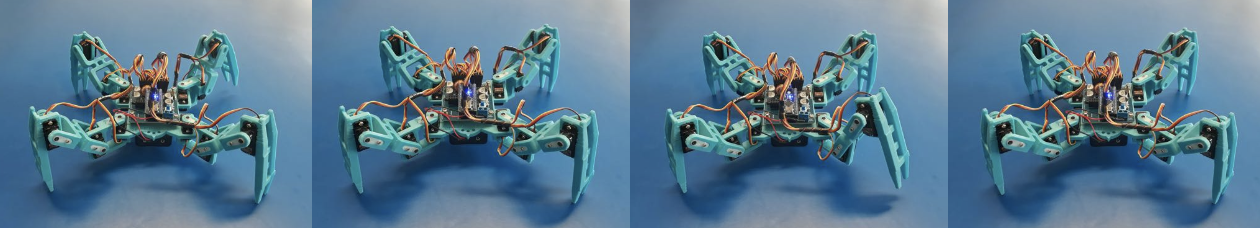
\includegraphics[width=0.8\textwidth]{./img/applaud_wave_2}
		\caption{Applaud sym}
	\end{center}
\end{figure}

applaud : tape une patte sur le sol

\begin{figure}[H]
	\begin{center}
		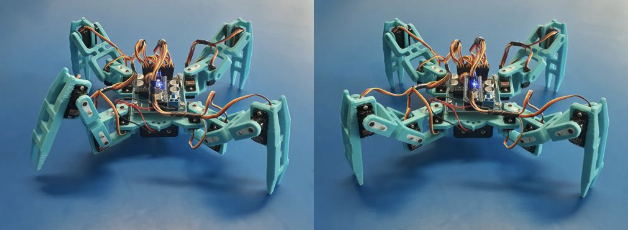
\includegraphics[width=0.3\textwidth]{./img/applaud}
		\caption{Applaud}
	\end{center}
\end{figure}

sputnik : lève les pattes en l'air

\begin{figure}[H]
	\begin{center}
		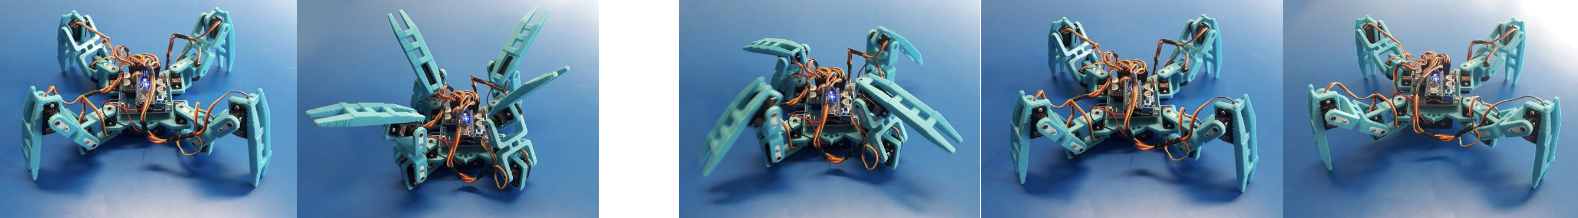
\includegraphics[width=0.8\textwidth]{./img/sputnik}
		\caption{Sputnik}
	\end{center}
\end{figure}

cross : étale les pattes sur le sol (en forme de croix)

\begin{figure}[H]
	\begin{center}
		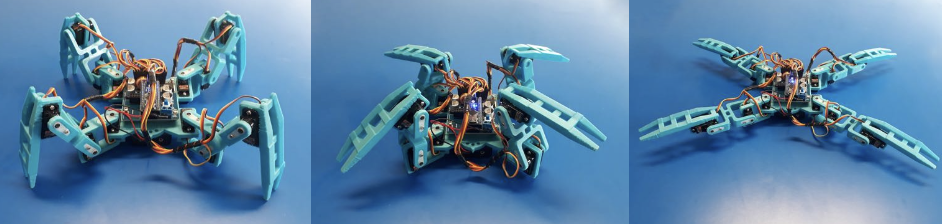
\includegraphics[width=0.8\textwidth]{./img/cross_1}
		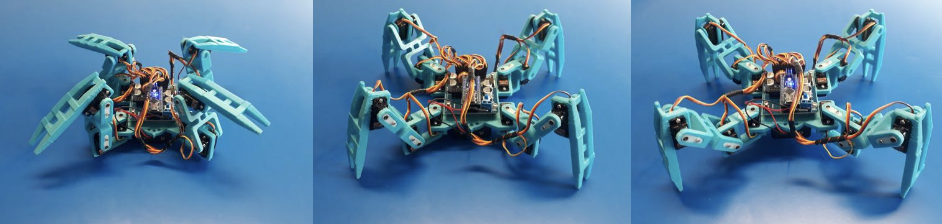
\includegraphics[width=0.8\textwidth]{./img/cross_2}
		\caption{Cross}
	\end{center}
\end{figure}

bolting : inspiré de la pose d'Usain Bolt : lève et étire deux pattes en diagonale

\begin{figure}[H]
	\begin{center}
		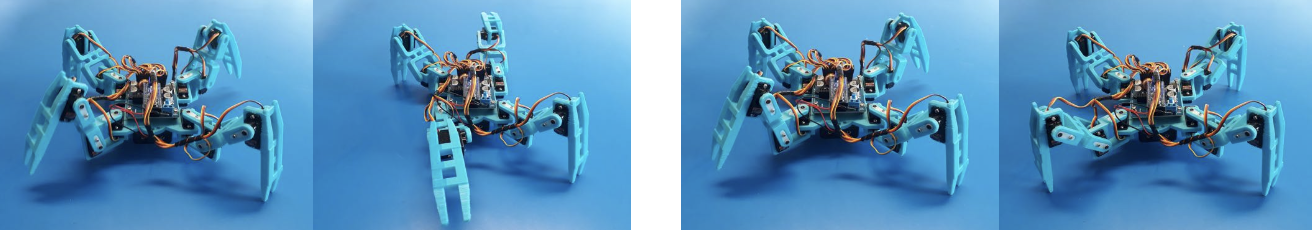
\includegraphics[width=0.8\textwidth]{./img/bolting}
		\caption{Bolting}
	\end{center}
\end{figure}

winx : simule un battement d'aile

\begin{figure}[H]
	\begin{center}
		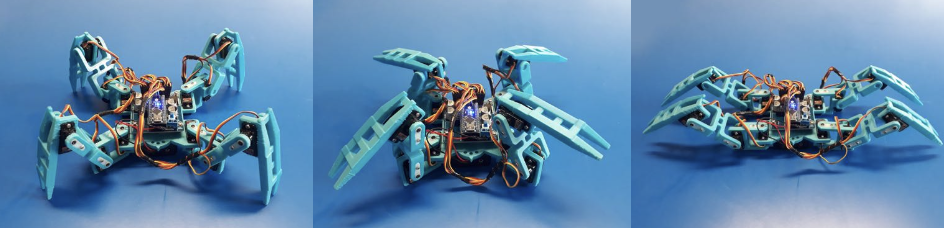
\includegraphics[width=0.6\textwidth]{./img/winx_1}
		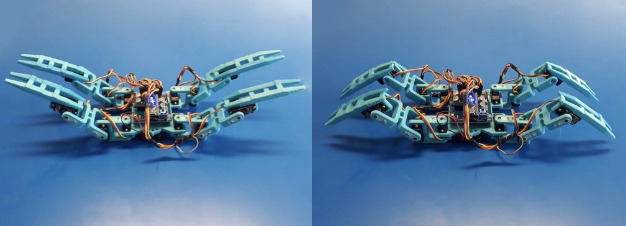
\includegraphics[width=0.6\textwidth]{./img/winx_2}
		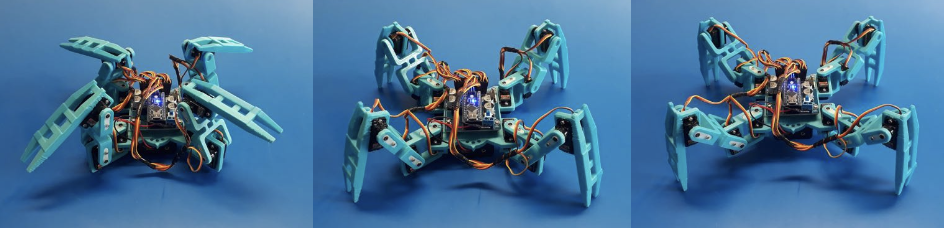
\includegraphics[width=0.6\textwidth]{./img/winx_3}
		\caption{Winx}
	\end{center}
\end{figure}

pls : position par défaut, araignée écrasée

\begin{figure}[H]
	\begin{center}
		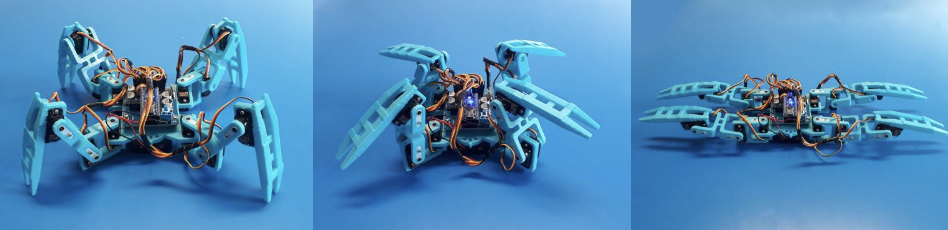
\includegraphics[width=0.6\textwidth]{./img/pls_1}
		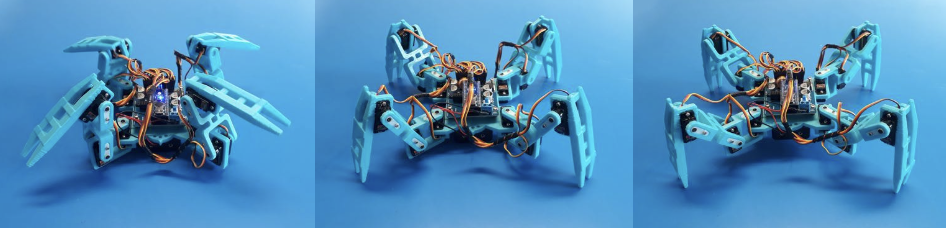
\includegraphics[width=0.6\textwidth]{./img/pls_2}
		\caption{PLS}
	\end{center}
\end{figure}

		%-----------------------
		\section{Synchronisation arraignées}
		%-----------------------

Nous avons testé la connexion wifi entre l'agent sur l'ordinateur et la carte en utilisant le code example de la librarie micro ROS :
\url{https://github.com/micro-ROS/micro_ros_arduino/blob/galactic/examples/micro-ros_publisher_wifi/micro-ros_publisher_wifi.ino}
L'exemple initie la connexion wifi et envoie un message à la carte.
Lorsque la connexion wifi échoue, la diode sur la carte se met à clignoter de manière intempestive.
\linebreak

Nous avons ensuite travaillé sur la synchronisation des arraignées : elles sont connectés par wifi à l'ordinateur qui envoient 
les messages en UDP.

		%-----------------------
		\section{Construction de la coque}
		%-----------------------

Pour modéliser notre coque nous avons utilisé OpenSCAD qui est un logiciel de modélisation 3D de type "constructif". 
Cela signifie que les modèles 3D sont créés en utilisant une syntaxe de script plutôt que par une interface graphique. 
OpenSCAD permet de créer des modèles 3D précis en combinant des primitives géométriques de base (par exemple, des cubes, des cylindres, 
des sphères) et en les modifiant à l'aide de transformations géométriques (par exemple, la rotation, la translation, l'échelle).  
\linebreak

Nous avions plusieurs idées de personnalisation de cette coque. La première idée était de faire un mini échiquier avec des petites 
pièces qui viendrait s’insérer par-dessus.  
La deuxième idée était d'ordre plus pratique. En effet, la carte Arduino que nous utilisons a besoin d’une source d’alimention 
en plus de celle déjà disponible sur l’araignée. Nous avons donc dû utiliser une batterie externe. 
L’idée était donc d’ajouter un socle qui pourrait tenir notre batterie sur l’araignée. 
\linebreak

Malheureusement, par manque de temps, nous avons dû nous contenter d’une coque plus basique qui nous permet cependant de 
faire tenir la batterie grâce à un élastique. 

\begin{figure}[H]
	\begin{center}
		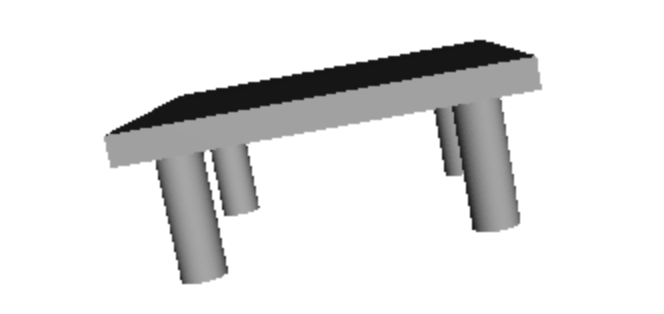
\includegraphics[width=0.3\textwidth]{./img/coque}
		\caption{Modèle 3D de la coque}
	\end{center}
\end{figure}


		%-----------------------
		\section{Limites et problèmes rencontrés}
		%-----------------------

Nous avons eu des soucis de compatibilité pour l'installation de ROS :  
\begin{itemize}
	\item[$\bullet$] sur Mac, il y avait un problème de dépendance python (graphviz) bien que la dépendance était installée
	\item[$\bullet$]sur Ubuntu 18.04, le framework ne fonctionnait pas (problème pour afficher une fenêtre graphique)
\end{itemize}

Pourtant d'après la documentation de ROS, le framework est censé pouvoir marcher sur ces OS et être cross-platform.
On notera que l'on peut également utiliser une image Docker pour ROS 2. 
\linebreak

Nous avons également dû utiliser l’IDE Platform IO (compatible Windows, Mac et Linux), une extension de VS Code, 
car impossible d'utiliser l'Arduino IDE car il manquait un time.h.
PlatformIO est designé pour faire marcher énormément de cartes et il faut donc spécifier la carte sur laquelle on travaille. 
Il se charge ensuite de récupèrer les libraries.
Nous avons ensuite installé l’agent Micro-ROS et testé le code de l’araignée SEALK pour tester les mouvements mais le code 
fourni ne marchait pas sur la carte. En effet, nous avions le problème de compilation suivant :  

\begin{lstlisting}
src/armcontroller.h:52:13: error: there are no arguments to 'sei' 
that depend on a template parameter, so a declaration of 'sei' 
must be available [-fpermissive]
sei();
\end{lstlisting}
Cette instruction permet d'activer les interruptions de timer.
Nous avons donc dû utiliser notre code que nous avons fait en cours avec les TP pour les mouvements de l'araignée.
\linebreak

Nous avons également dû utiliser la librarie suivante pour faire marcher correctement les servomoteurs : RP2040\_ISR\_Servo (\url{https://github.com/khoih-prog/RP2040_ISR_Servo}).
En effet, les mouvements envoient une instruction en dehors de la loop principale.
